\section{Introduction}
\label{sec:intro}

A normal Magic card has five main parts which I examine. In the top left corner
is the card's \textbf{name}, the upper middle is the card's \textbf{art}, 
the text immediately below the image is the card's \textbf{type}, and finally, 
the \textbf{color} of the card is depicted by the color surrounding it all. 
As an example, refer to figure \ref{fig:intro_card}.
\begin{figure}[h!]
    \centering
    \begin{subfigure}[b]{0.6\linewidth}
        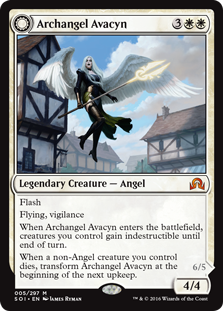
\includegraphics[width=\linewidth]{figures/card.png}
        \caption{Archangel Avacyn}
    \end{subfigure}
    \begin{subfigure}[b]{0.6\linewidth}
        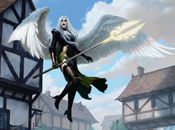
\includegraphics[width=\linewidth]{figures/ArchangelAvacynCut.png}
        \caption{Just the Art}
    \end{subfigure}
    \caption{A card and its art}
    \label{fig:intro_card}
\end{figure}

\noindent
Let
\[ Colors=\left\{\ \parbox[c]{.6\linewidth}{%\raggedright%
white, black, red, green, blue, $\varepsilon$
}\ \right\}
\]
\[ Types=\left\{\ \parbox[c]{.65\linewidth}{%\raggedright%
creature, land, instant, sorcery, enchantment, artifact, planeswalker
}\ \right\}
\]

Every card has a set of colors $c \subset Colors$ 
and every card has a singular type $t \in Types$.
So for the example in figure one, we would have a table
like the one below.
\indent

\begin{table}[h!]
    \begin{center}
        \label{tab:intro_card_table}
        \begin{tabular}{l|c}
            \textbf{Piece} & \textbf{Instance} \\
            \hline
            Name & Archangel Avacyn \\
            Type & Creature \\
            Color & white \\
            Art & figure (b)
        \end{tabular}
    \end{center}
\end{table}

Now that all of the pieces of a Magic card have their place,
we can think of what to do with them. For my project, I looked
at the ability of a neural net to predict a piece P, given some
set of the remaining pieces. The first effort I made was in predicting 
the color of a card, given its name. In Magic the Gathering, each
color has themes that relate to it. For example, Green is synonymous
with life and large monsters (like dinosaurs), while Blue is connected
to wizards who casts spells. I hope to discover a corrolation between
the name of a card and the theme of a card, which would then be used
to predict the color. Similarly, I will attempt to predict the type
of a card using the name. Finally, I experiment with Convolutional 
Neural Networks to predict these same features using the artwork
on a card.
